\documentclass[reprint,floatfix,amsmath,amssymb,aps,pra]{revtex4-1}

\usepackage{dragly-revtex}

\usepackage{}

\begin{document}

\title{FYS4460 Project 1}
\author{Svenn-Arne Dragly}

\begin{abstract}
In this project we study a monatomic gas consisting of Argon atoms using molecular dynamics.
\end{abstract}

\maketitle

\section{Introduction}

\section{Theory}

\subsection{Integration}

We assume that our particles adhere to Newtonian motion based on the interatomic forces and use the velocity-Verlet method to integrate motion in our system.

\subsection{Interatomic force}

The interatomic force is based on a chosen Lennard-Jones potential.
\begin{equation}
    V_{LJ} = 4 \varepsilon \left[ \left( \frac {\sigma} {r} \right)^{12} - \left( \frac {\sigma} {r} \right)^6 \right]
\end{equation}
where $r$ is the distance between two atoms, $\sigma$ is chosen to be $\sigma = 3.405 \unit{\AA}$ and $\varepsilon = 1.0318 \cdot 10^{−2} \unit{eV}$.

Taking the gradient of the potential gives us the force as
\begin{equation}
 \vec F = \frac{24 \varepsilon}{r^{2}} \left[ \left( 2 \frac {\sigma} {r} \right)^{12} - \left( \frac {\sigma} {r} \right)^6 \right] \vec r
\end{equation}

\section{Implementation}

\subsection{Periodic boundary conditions}

Our system is limited in size, but to 

\subsection{Neighbor cells}

To make the calculations go faster, we decide on a cutoff distance for the force. Outside this cutoff distance, we assume that the interatomic force is zero. Inside, it is still defined by the Lennard-Jones potential. In this project, we set the cutoff distance to be $r_{\text{cut}} = 3 \sigma$.

To make use of this, we implement neighbor cells\footnote{Neighbor cells are generally easier to combine with parallel code. Another approach is to use Verlet lists.} as a division of our space into regions at least as large as $r_{\text{cut}}$ in all directions.

\section{Results}

\subsection{Boltzmann distribution of velocities}

\begin{figure*}
    \centering
    \subfigure[]{
        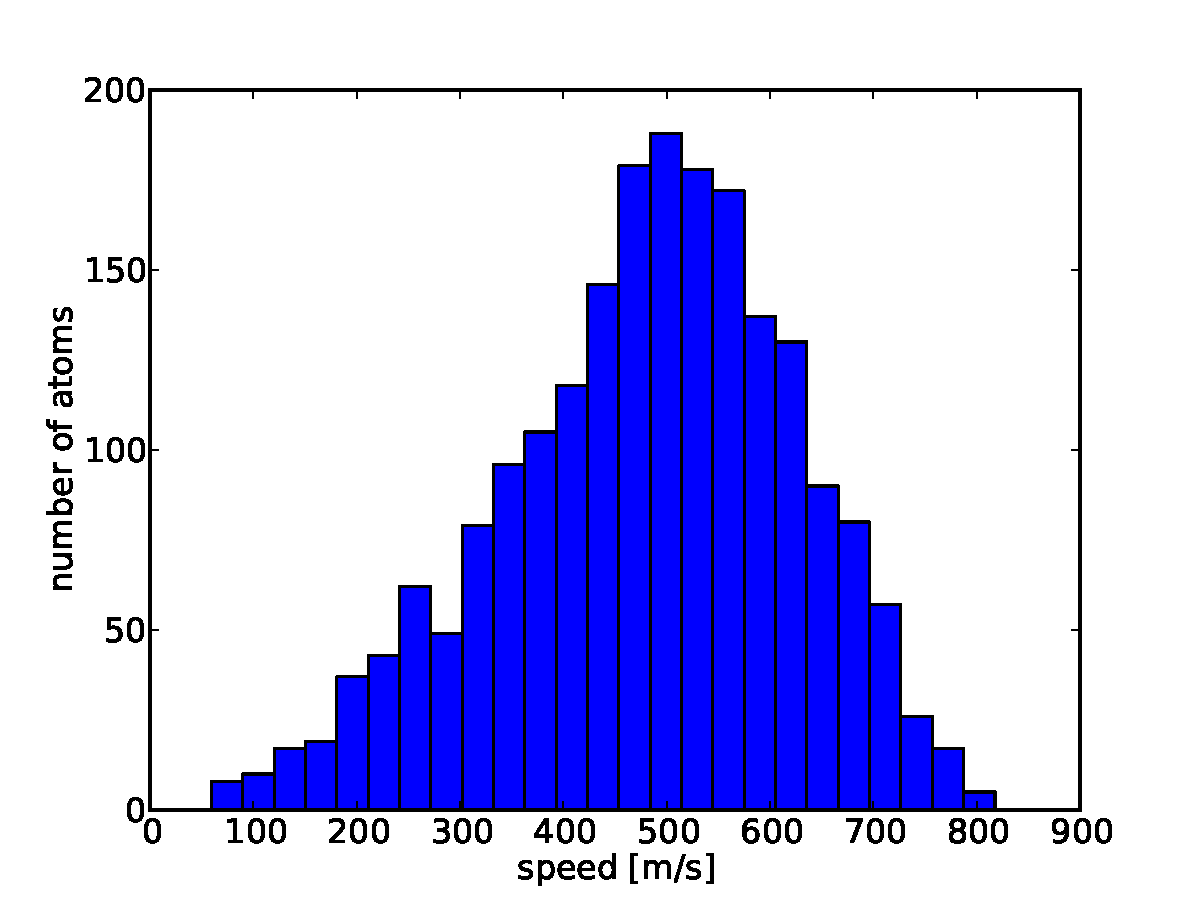
\includegraphics[width=0.48\textwidth]{./analysis/1i-boltzmann/runs/2013-02-26_180246/data000000-norm.pdf}
    } \label{fig:velocity-magnitudes}
    \subfigure[]{
	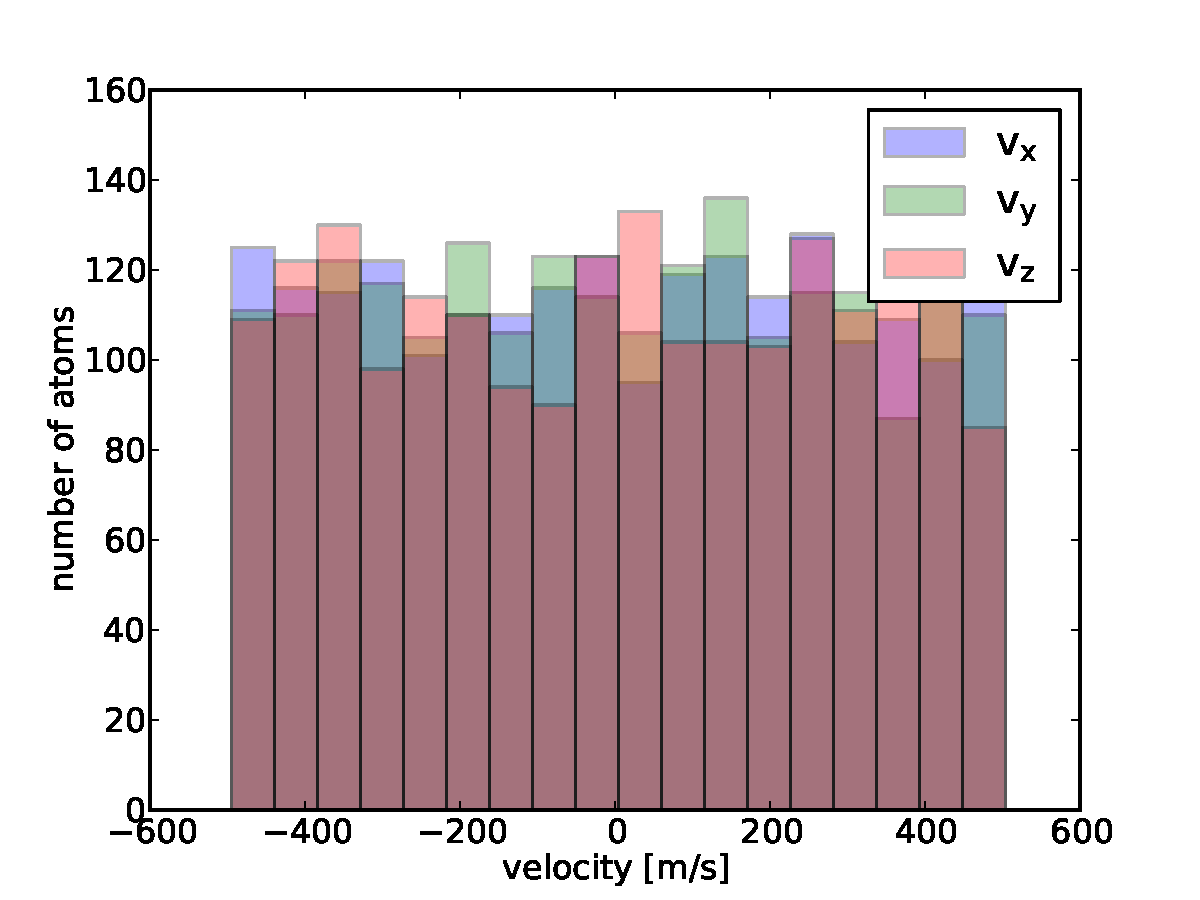
\includegraphics[width=0.48\textwidth]{./analysis/1i-boltzmann/runs/2013-02-26_180246/data000000-comp.pdf}
    } \label{fig:velocity-magnitudes}
    % fitness0.pdf: 576x432 pixel, 72dpi, 20.32x15.24 cm, bb=0 0 576 432
    \caption{Magnitudes (a) and components (b) of the velocities in the first timestep after initializing with random uniform velocities in each direction, showing a non-Boltzmann distribution.}
    \label{fig:velocity-evolution}
\end{figure*}

\begin{figure*}
    \centering
    \subfigure[]{
        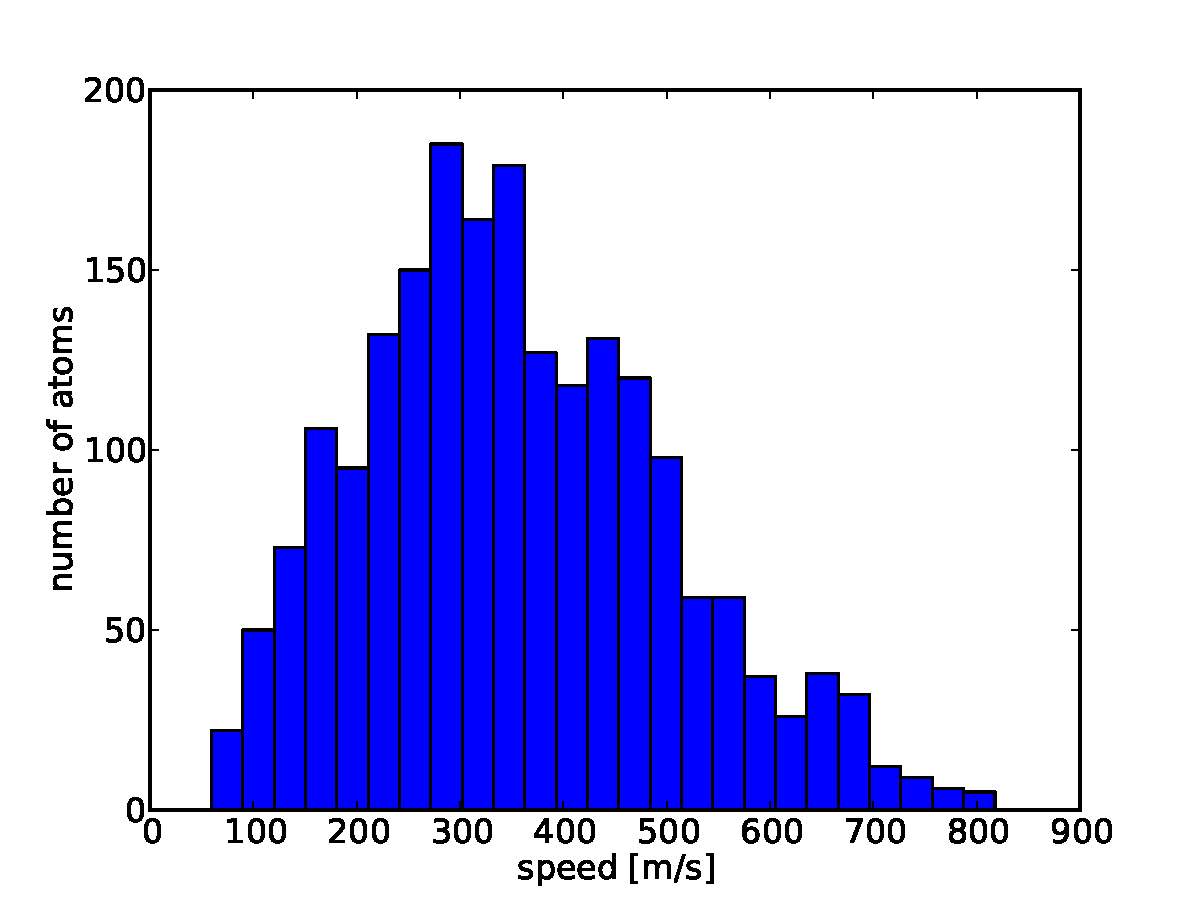
\includegraphics[width=0.48\textwidth]{./analysis/1i-boltzmann/runs/2013-02-26_180246/data000095-norm.pdf}
    } \label{fig:velocity-magnitudes}
    \subfigure[]{
	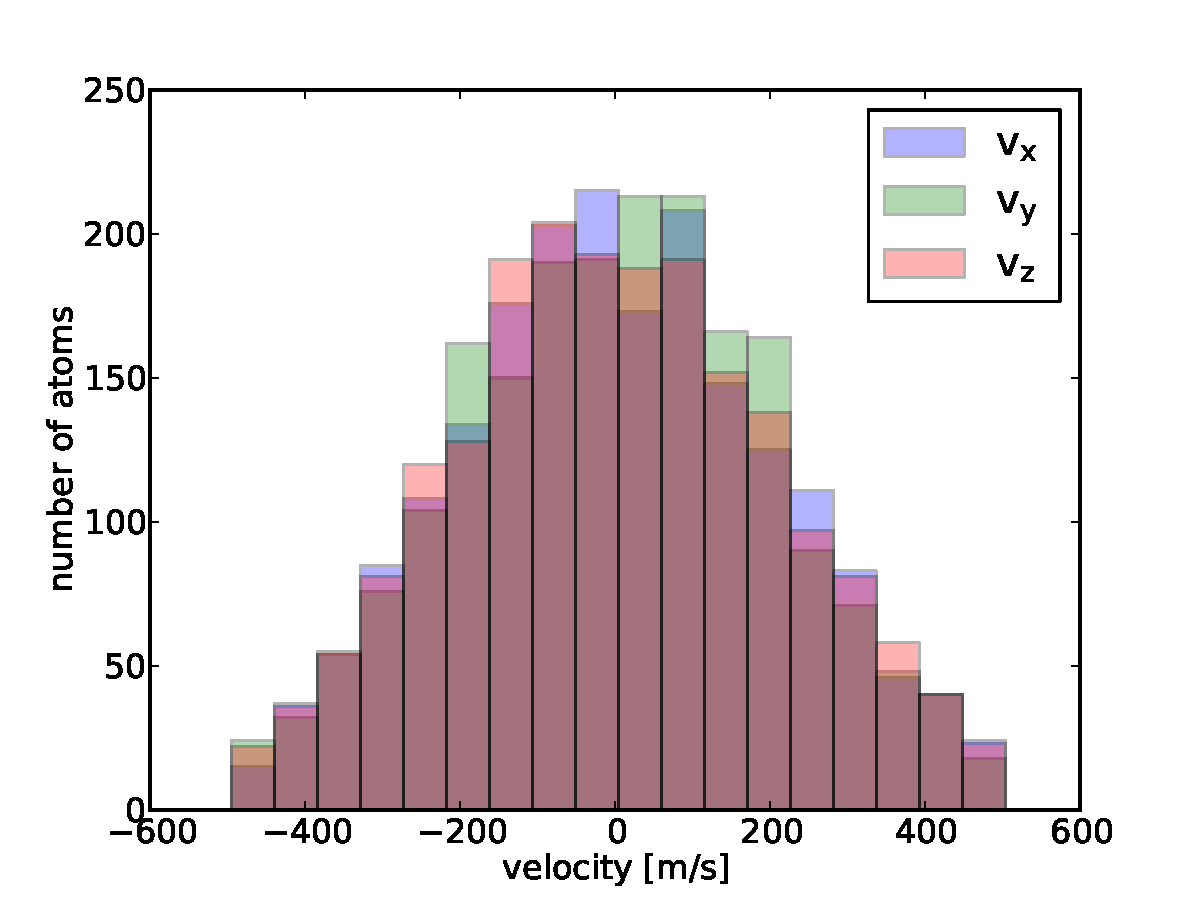
\includegraphics[width=0.48\textwidth]{./analysis/1i-boltzmann/runs/2013-02-26_180246/data000095-comp.pdf}
    } \label{fig:velocity-magnitudes}
    % fitness0.pdf: 576x432 pixel, 72dpi, 20.32x15.24 cm, bb=0 0 576 432
    \caption{Magnitudes (a) and components (b) of the velocities 100 timesteps after initializing with random uniform velocities in each direction. This clearly shows a Boltzmann distribution of the magnitudes and a normal distribution of the components.}
    \label{fig:velocity-evolution}
\end{figure*}

\subsection{Energy fluctuations}

\begin{figure*}
    \centering
    \subfigure[~ $\Delta t = 1.2 \cdot 10^{-14} \unit{s}$]{
        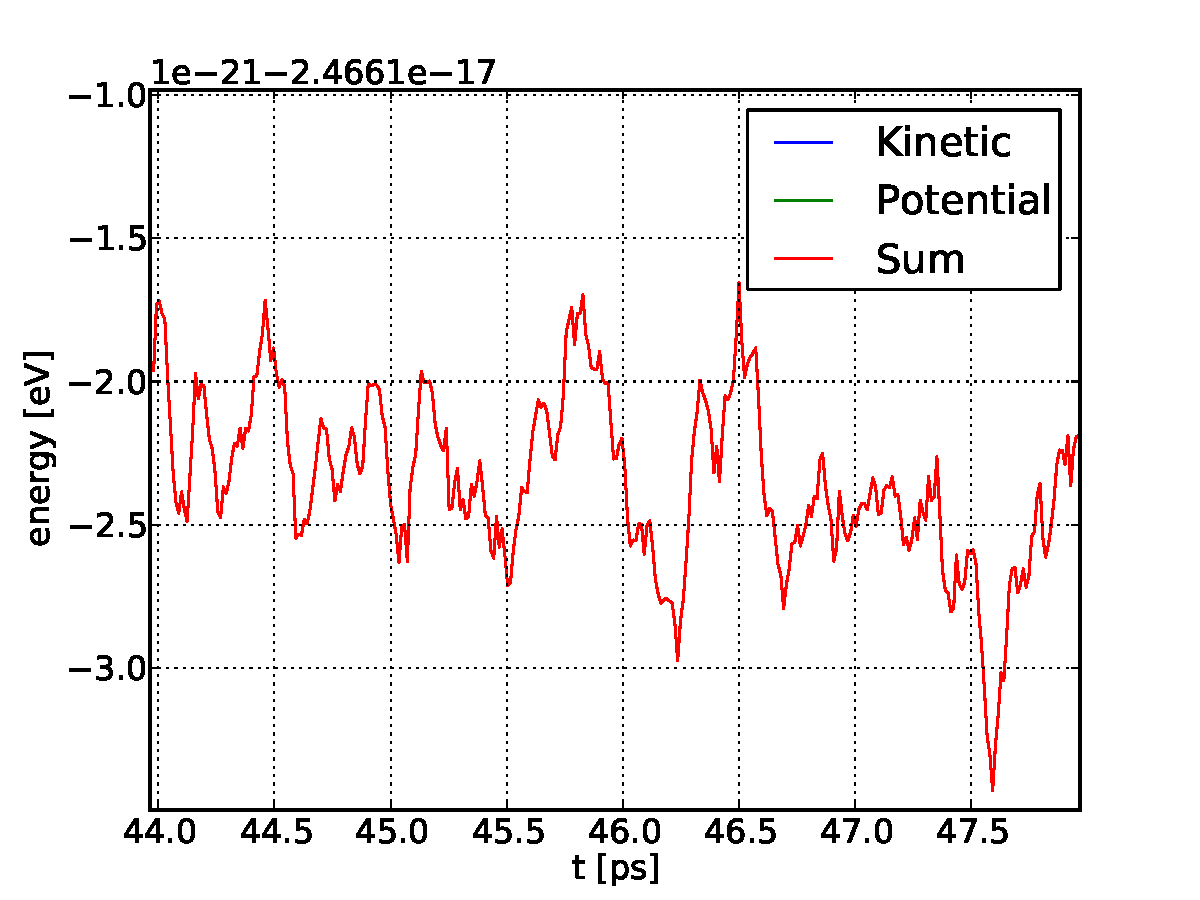
\includegraphics[width=0.48\textwidth]{./analysis/1j-energy/runs/2013-02-25_140300/energy-0001.pdf}
    } \label{fig:velocity-magnitudes}
    \subfigure[~ $\Delta t = 5.6 \cdot 10^{-14} \unit{s}$]{
        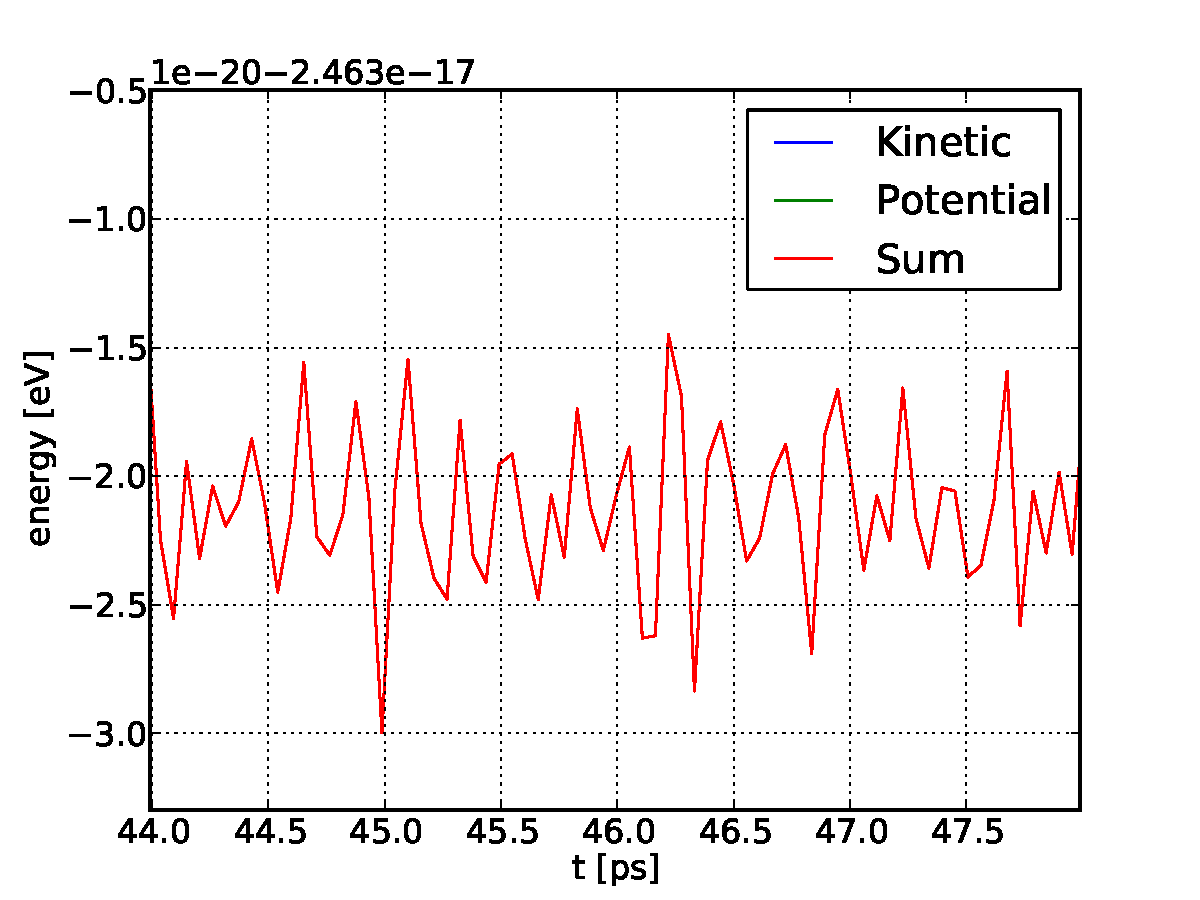
\includegraphics[width=0.48\textwidth]{./analysis/1j-energy/runs/2013-02-25_140300/energy-0005.pdf}
    } \label{fig:velocity-magnitudes}
    % fitness0.pdf: 576x432 pixel, 72dpi, 20.32x15.24 cm, bb=0 0 576 432
    \caption{Fluctuations in kinetic energy as for a small timestep (a) and a large timestep (b).}
    \label{fig:velocity-evolution}
\end{figure*}

% \begin{figure}
%  \centering
%  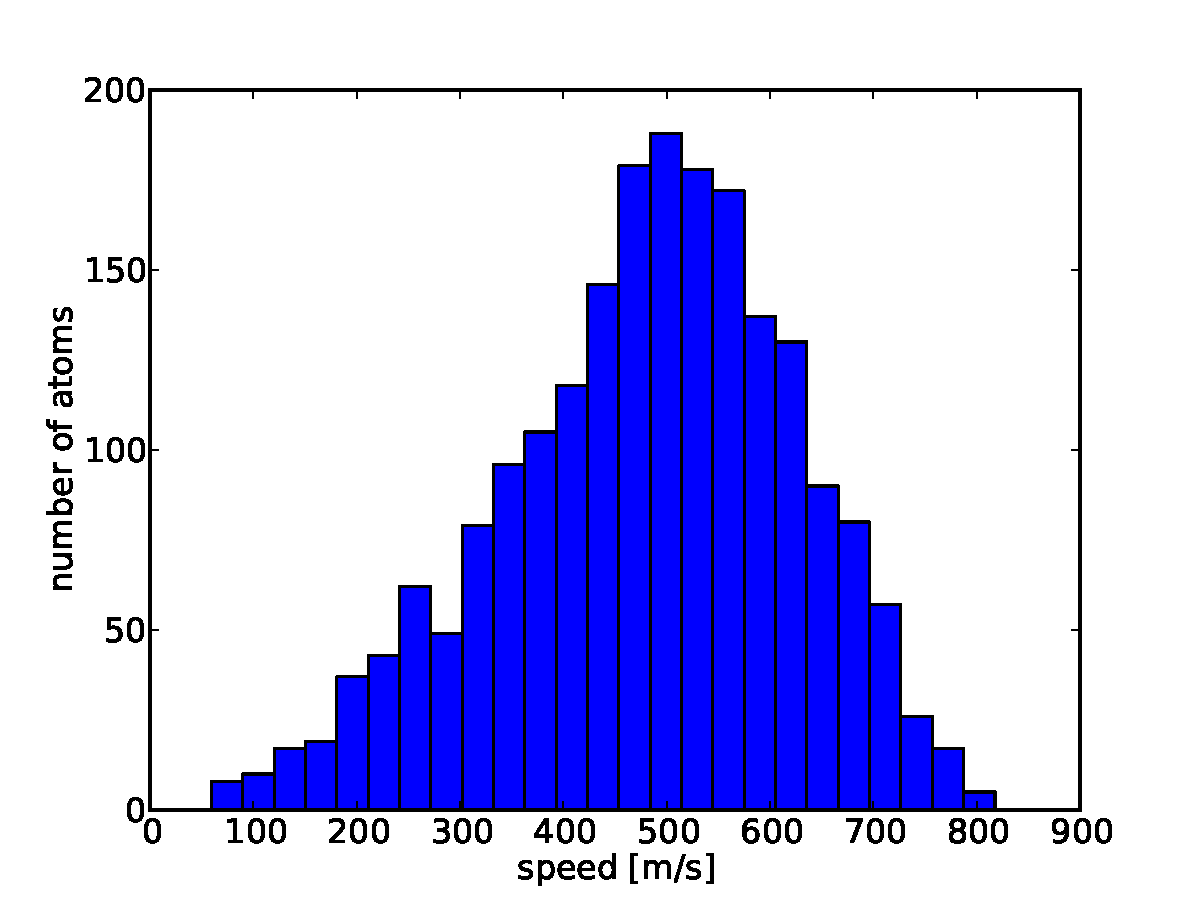
\includegraphics[width=0.5\textwidth]{./analysis/1i-boltzmann/runs/2013-02-26_180246/data000000-norm.pdf}
%  % data000000.bin-norm.pdf: 576x432 pixel, 72dpi, 20.32x15.24 cm, bb=0 0 576 432
%  \caption{Magnitudes of the velocities in the first timestep after initializing with random uniform velocities in each direction, showing a non-Boltzmann distribution.}
%  \label{fig:velocity-magnitudes}
% \end{figure}
% \begin{figure}
%  \centering
%  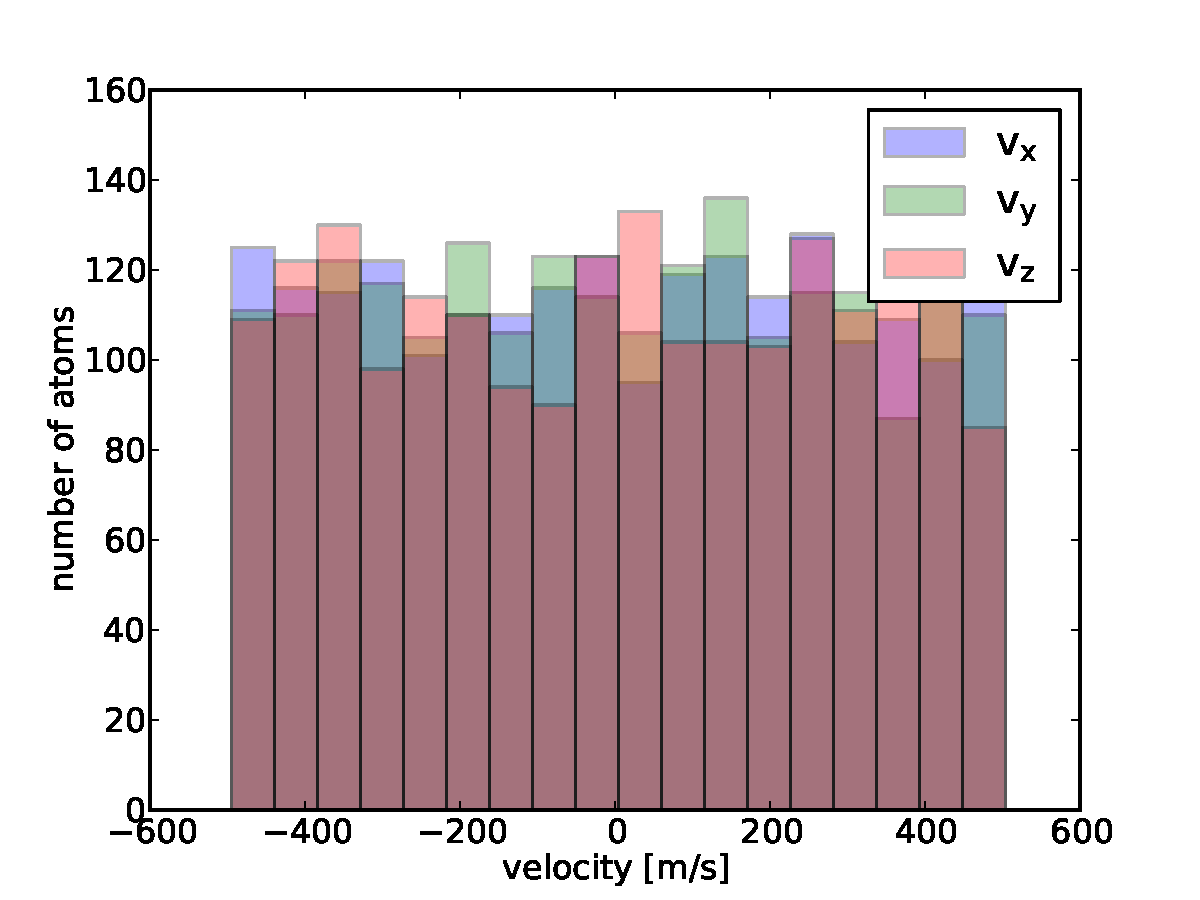
\includegraphics[width=0.5\textwidth]{./analysis/1i-boltzmann/runs/2013-02-26_180246/data000000-comp.pdf}
%  % data000000.bin-norm.pdf: 576x432 pixel, 72dpi, 20.32x15.24 cm, bb=0 0 576 432
%  \caption{Components of the velocities in the first timestep after initializing with random uniform velocities in each direction, showing a non-Boltzmann distribution.}
%  \label{fig:velocity-magnitudes}
% \end{figure}



\appendix

\section{Conversion to atomic units}

\bibliographystyle{abbrvnat}
\bibliography{references}

\end{document}
